\documentstyle[12pt,epsfig]{article}
\setlength{\unitlength}{1.cm}
\doublerulesep -1pt 
\textwidth=6.5in 
\textheight=9.5in
\hoffset=-1cm 
\voffset=-1in 
\pagestyle{empty}
\begin{document}

\begin{center}
{\bf\sc Massachusetts Institute of Technology}\\
{\bf\sc Experimental Study Group}\\
{\bf\sc 8.022 Spring 2011}\\
\bigskip
{\bf\sc Optional problems: Special relativity}\\
%Post date: Wednesday, March 16th\\
%Due date: Wednesday, March 30th\\
%Be sure to write your {\bf name} and {\bf section number} on your
%pset\\
%Please {\bf staple} multiple pages together
\end{center}

\begin{enumerate}

\item Lenght contraction. Measure the length of a train car in the train reference frame and
 in the station reference frame. How are they related?
 Hint: Place a light source at the back of a train and a mirror at the front.
 The train  moves with constant velocity $\vec v= v\hat{x}$. We flash the light in the forward direction where
  it reflects and returns to the back of the train. What are the travel times in the two reference
   frames in consideration?

\item Invariant interval (8 pts): A quantity that is left unchanged by
Lorentz transformations is called a ``Lorentz invariant''.  Consider
two events described in the laboratory frame by ($t_1, x_1, y_1, z_1$)
and ($t_2, x_2, y_2, z_2$).  Show that
\begin{eqnarray*}
\Delta s^2 \equiv -(c\Delta t)^2 + (\Delta x)^2 + (\Delta y)^2 +
(\Delta z)^2
\end{eqnarray*}
is a Lorentz invariant.

\item Galilean tranformations (10 pts): Prior to special relativity,
people related coordinates between different frames with the
``Galilean transformation'' --- clocks in different reference frame
tick at the same rate, spatial positions are shifted by a term that
depends on the relative velocity just as you would expect.  For
example, for frames that are moving with respect to each other in the
$x$ direction, we would have
\begin{eqnarray*}
t' &=& t
\\
x' &=& x - v t\;.
\end{eqnarray*}
Using the binomial expansion on $\gamma$, show that for small $v/c$
the Lorentz tranformations reduce to the Galilean tranformations.  At
what value of $v$ does the next term in the expansion change the $x$
transformation by $1\%$?

\item Transforming velocities (15 pts): A bullet is fired with
velocity $\vec u'$ in the $(x',y')$ plane of a moving frame $F'$.
Frame $F'$ moves with speed $v$ in the $+x$ direction with respect to
the laboratory frame $F$.

\par\noindent (a) [6 pts] Find the angle that the velocity vector makes
with $x$ axis of the lab frame.

\par\noindent (b) [3 pts] What is this angle in the limit $|\vec u'| =
c$?  Does anything wierd happen?

\par\noindent (c) [6 pts] Show that when $|\vec u'| = c$, $|\vec u| =
c$ --- the speed of light is the same in both frames.

%\begin{center}
%{\it Go to page 2...}
%\end{center}

\newpage

\item ``Beating the speed of light'' (20 pts): Your crazy uncle is fed
up with all this fancy book learnin' you're getting at MIT.  He's
particularly unhappy that you're studying special
relativity.  He claims
that he can build a device that will easily disprove the idea that
nature has a speed limit (i.e., that nothing can go faster than the
speed of light).

The idea is as follows.  We make a cart roll across the floor with
speed $v$.  We put a smaller cart on top of that cart, and roll it
with speed $v$ {\it with respect to the first cart}, and in the same
direction as the first cart.  We put a third cart on this second cart;
it rolls with speed $v$ {\it with respect to the second cart}.  We put
a fourth cart ... you get the idea.  Your uncle claims that there is
some $n$ at which the cart must be going faster than the speed of
light.

\begin{figure}[ht]
\begin{center}
\includegraphics[width = 12cm]{cart.eps}
\end{center}
\end{figure}

\par\noindent (a) [10 pts] Prove him wrong.  Using mathematical
induction, prove that if $v < c$, then $v_n < c$, where $v_n$ is the
velocity of the $n$th cart.  Show that this holds even for extremely
large $n$.

\par\noindent (b) [10 pts] Calculate the value of $v_n$ given $v$ and
$n$.  To facilitate this, note the following very useful identity:
\begin{eqnarray*}
\tanh(a + b) = \frac{\tanh(a) + \tanh(b)}{1 + \tanh(a)\tanh(b)}\;
\end{eqnarray*}
Define $v_n = c \tanh x_n$.  Using the above formula and comparing to
the special relativity rule for adding velocities, first work out how
$x_n$ adds, then deduce $v_n$.  What is $v_\infty$?

\item Energy-momentum identity (7 pts): Show that
\begin{eqnarray*}
E^2 = p^2 c^2 + m^2 c^4
\end{eqnarray*}
where $p = |\vec p|$.


\newpage


\item Transformation of fields (15 pts): A very large sheet of charge
lies in the $x-y$ plane of the frame $F$.  The charge per unit area of
this sheet is $\sigma$.  In the frame $F'$, this sheet moves to the
right with speed $v$.

\par\noindent (a) [3 pts] What is the electric field in the rest
frame (above and below the sheet)?

\par\noindent (b) [4 pts] What is the electric field in the frame $F'$
(above and below the sheet)?

\par\noindent (c) [5 pts] What is the magnetic field in the frame $F'$
(above and below the sheet)?  (To do this, first think of what kind of
current must come from a moving sheet of charge.  Dimensional analysis
should help you here.)

\par\noindent (d) [3 pts] Show that the results of (b) and (c) are
consistent with the general Lorentz transformations for electric and
magnetic fields, Eq.\ (60) of Purcell Chapter 6.

\end{enumerate}

\newpage

8.

\begin{figure}[h!]
\begin{center}
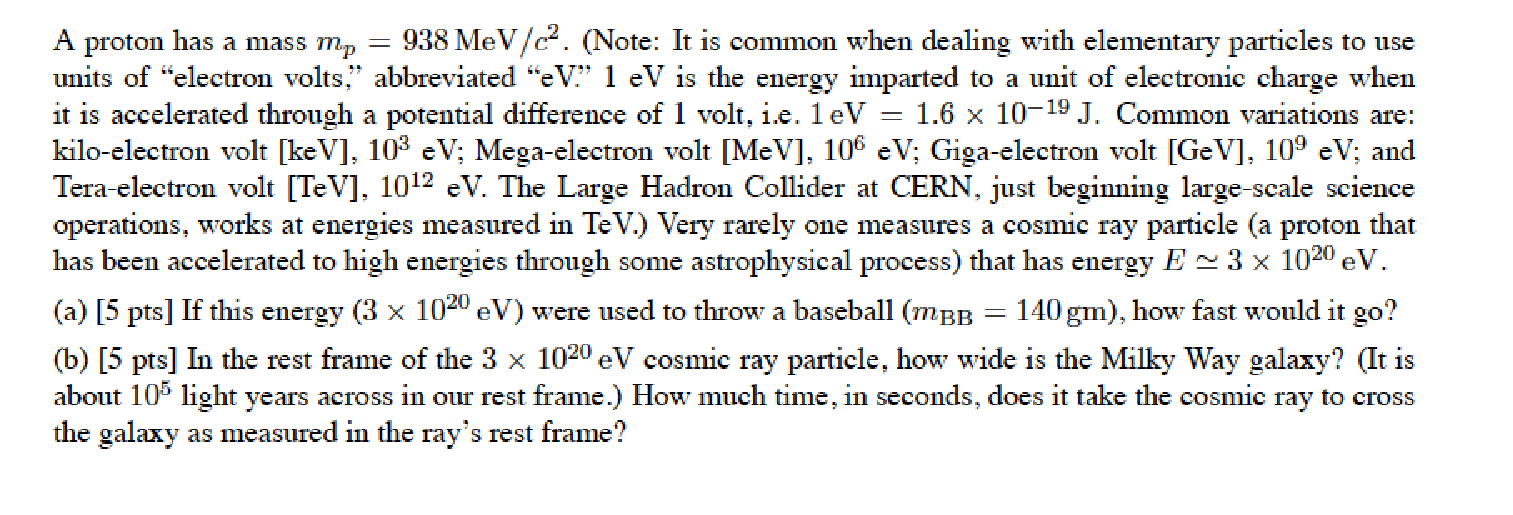
\includegraphics[width = 12cm]{cosmic_rays.eps}
\end{center}
\end{figure}

9.

\begin{figure}[h!]
\begin{center}
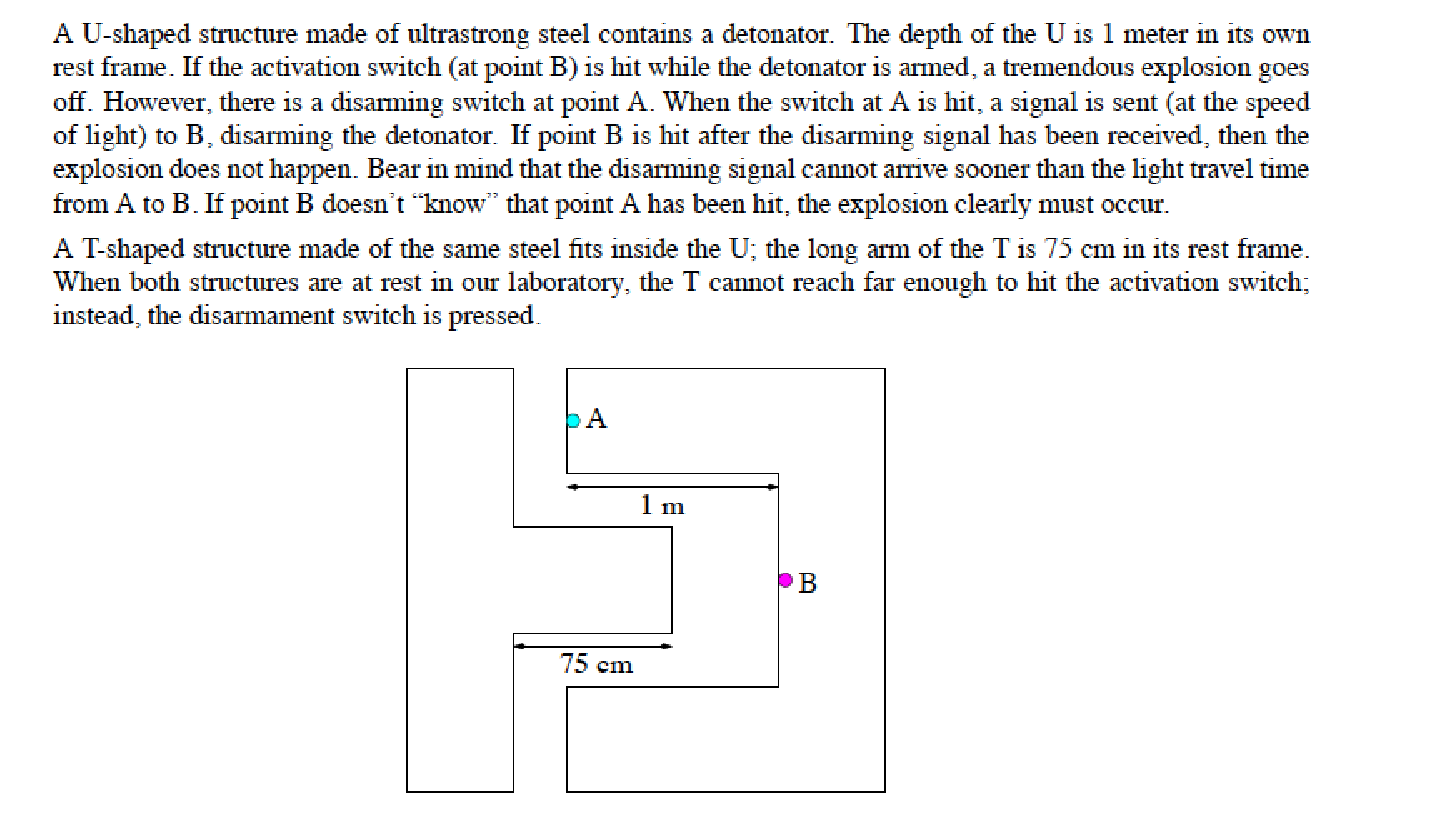
\includegraphics[width = 12cm]{paradox_1.eps}
\end{center}
\end{figure}

\begin{figure}[h!]
\begin{center}
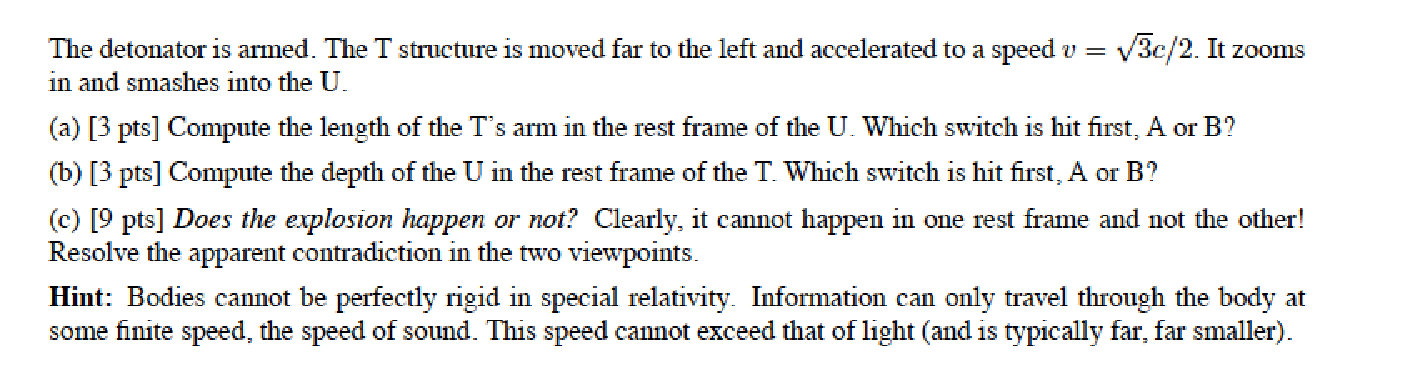
\includegraphics[width = 12cm]{paradox_2.eps}
\end{center}
\end{figure}



\end{document}
